% filepath: PID-in-Modern-Cherenkov/Sections/pid-via-thetac.tex
% Content for the "PID via \theta_c Measurement" subsection

PID in Cherenkov imaging detectors principally requires the measurement of the Cherenkov angle of a particle at a known momentum. Using the relativistic transformations for momentum and energy
\begin{align}
\label{equ:relativistic-momentum}
p &= \gamma m_{0} v      \\
\label{equ:relativistic-energy}
E &= \gamma m_{0} c^2   
\end{align} 
we can rewrite the Cherenkov angle from Equ \nolinebreak\ref{equ:cherenkov-angle} as
\begin{equation}
\cos{\theta_c} = \frac{\sqrt{p^2 + m^2c^2}}{np}\; .
\label{equ:cherenkov-angle-relativistic}
\end{equation}
At a fixed momentum, the Cherenkov angle provides separation between particle hypotheses with different masses. 
This equation can be used to plot the analytical curves for the experimental data in Fig \nolinebreak\ref{fig:cherenkov-angle-clas12}.

\begin{figure}[h]
\centering
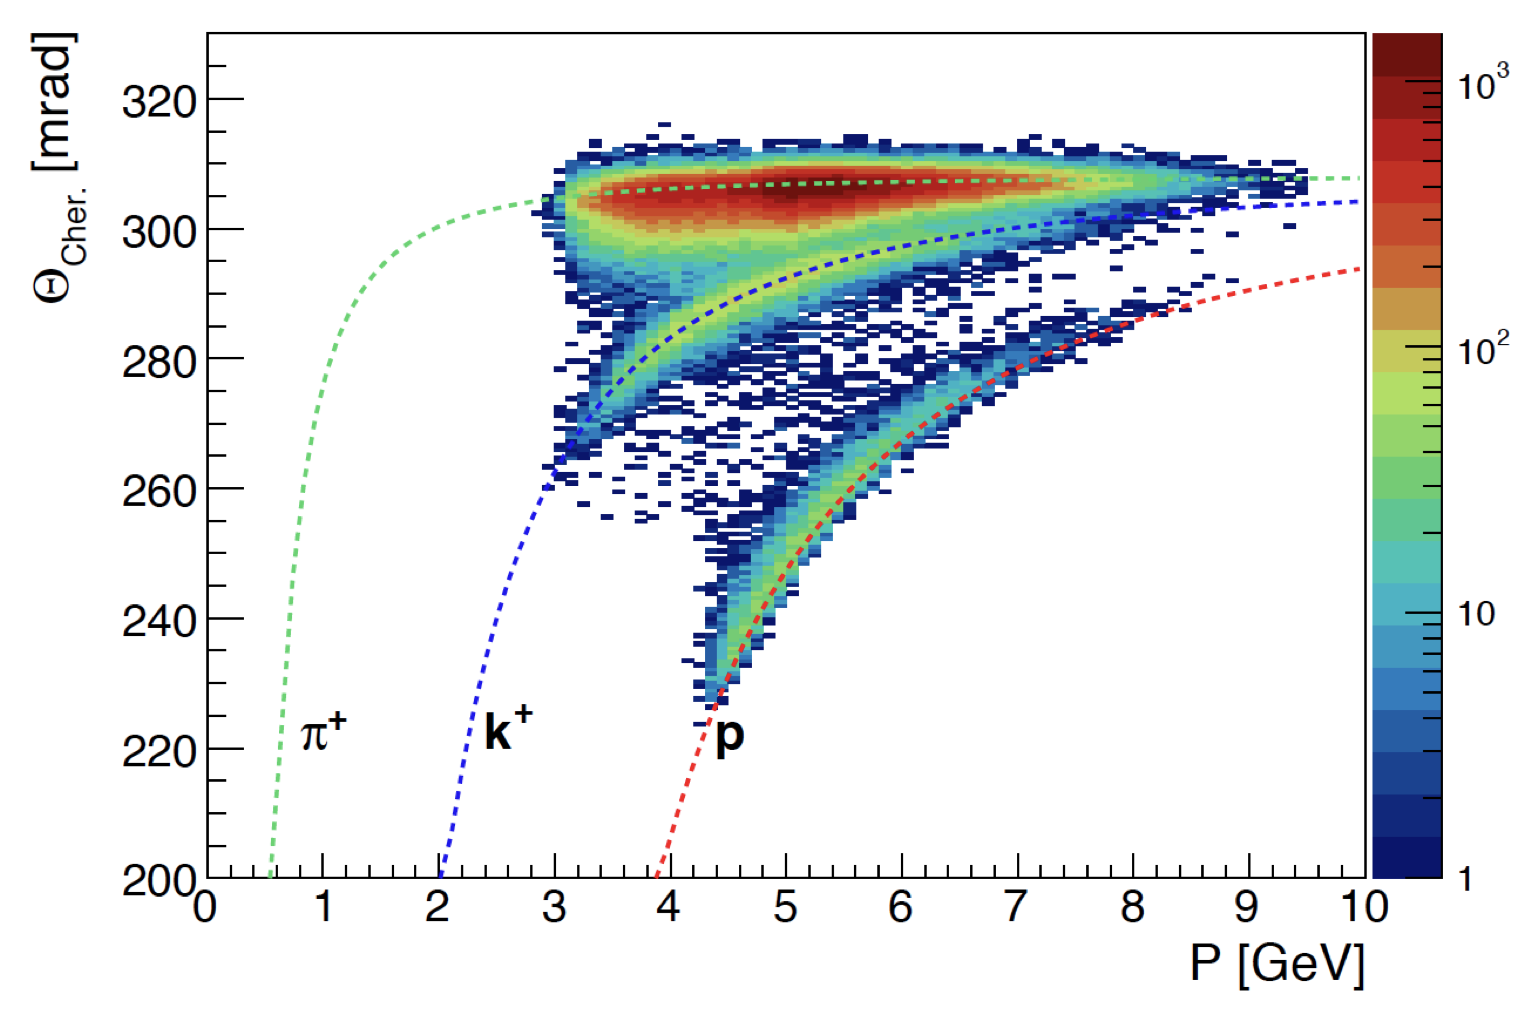
\includegraphics[width=\linewidth]{Images/cherenkov-angle-clas12.png}
\caption{\textbf{Cherenkov angle response of the CLAS12 detector at JLab \nolinebreak\cite{CONTALBRIGO2020163791}.} There are distinct curves for different particle species. The analytical form of these curves can be determined using Equ \nolinebreak\ref{equ:cherenkov-angle-relativistic}. \label{fig:cherenkov-angle-clas12}}
\end{figure}

In modern detector arrays at collider setups, forward tracking detectors provide momentum measurements. Then, Cherenkov track-based PID detectors (such as RICHs in Sect \nolinebreak\ref{sec:rich})
provide measurement of the Cherenkov angle through analysis of the Cherenkov photon hits
incident on a photodetector array. 
Large-volume detectors (such as Super-K in Sect \nolinebreak\ref{sec:neutrino-identification})
map the entire Cherenkov cone of photons using photodetectors over a huge area, and can obtain momentum estimates
from the light intensity. 
